\documentclass[12pt]{minimal}

\usepackage{graphicx}
\graphicspath{ {paper_figures2/} }

\usepackage{tikz}

%\usepackage[margin=0in, paperwidth=8.7cm, paperheight=9.5cm]{geometry}
\usepackage[margin=0in, paperwidth=8.7cm, paperheight=11.7cm]{geometry}

\begin{document}

\centering
\begin{tikzpicture}
	\node at (0cm, 0cm) {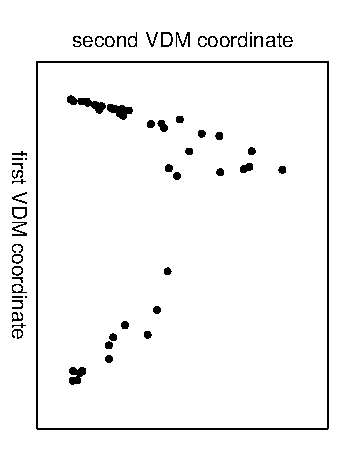
\includegraphics[width=6.9cm, angle=90]{data3_embed_bw}};
	\node at (-4.35cm, 2.75cm) {\textsf{A}};
	%\draw[help lines,step=.5] (-4,-4) grid (4,4);
	\draw [draw=white!50!gray, ->, ultra thick] (-2.2, -2) .. controls (-1.1, 0.5) and  (1, 0)  .. (2, -2);
	\draw [draw=white!50!gray, ->, ultra thick] (-3, -1.8)  .. controls (-2.6, 0.9) and (-1.9, 1.5) .. (-1.7, 2.1); 
	\node at (2.05cm, 1.6cm) {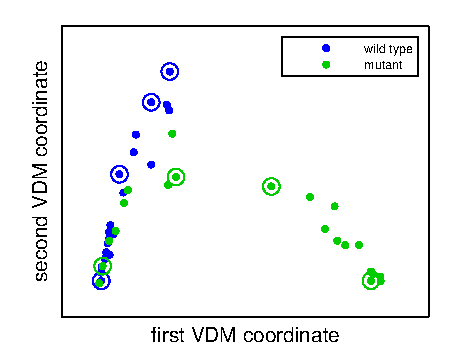
\includegraphics[width=4.1cm]{data3_embed_color}};
\end{tikzpicture}\\
\begin{tikzpicture}
	\node at (-4.25cm, 0cm) {\textsf{B}};
	\node at (0,0) {
\includegraphics[width=8cm]{wt_trajectory}};
	%\draw[help lines,step=.5] (-4,-1) grid (4,1);
	\draw[->, color=white, thick] (-1.1cm, -0.1cm) -- (-1.3cm, -0.3cm);
	\draw[->, color=white, thick] (-0.7cm, -0.1cm) -- (-0.5cm, -0.2cm);

	\draw[->, color=white, thick] (0.75cm, -0.1cm) -- (0.6cm, -0.3cm);
	\draw[->, color=white, thick] (1.25cm, -0.1cm) -- (1.4cm, -0.3cm);
	
	\draw[->, color=white, thick] (2.8cm, -0.1cm) -- (2.7cm, -0.3cm);
	\draw[->, color=white, thick] (3.3cm, -0.1cm) -- (3.5cm, -0.3cm);

\end{tikzpicture}\\
\begin{tikzpicture}
	\node at (-4.25cm, 0cm) {\textsf{C}};
	\node at (0,0) {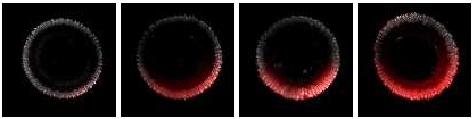
\includegraphics[width=8cm]{mut_trajectory}};

	\draw[->, color=white, thick] (-1cm, -0.2cm) -- (-1cm, -0.5cm);
	
	\draw[->, color=white, thick] (1cm, -0.2cm) -- (1cm, -0.5cm);
	
	\draw[->, color=white, thick] (3cm, -0.2cm) -- (3cm, -0.5cm);

\end{tikzpicture}

\end{document}